%!TEX root=../ctl-phd-thesis.tex

\section{Abstract}
Allosteric drug development holds promise for delivering medicines that are more selective and less toxic than those that target orthosteric sites. To date, the discovery of allosteric binding sites and lead compounds has been mostly serendipitous, through high-throughput screening. Over the last decade, structural data has become readily available for larger protein systems and more membrane protein classes (e.g., GPCRs and ion channels), which are common allosteric drug targets. In parallel, improved simulation methods now provide better atomistic understanding of the protein dynamics and cooperative motions that are critical to allosteric mechanisms. As a result of these advances, the field of predictive allosteric drug development is now on the cusp of a new era of rational structure-based computational methods. Here, we review algorithms that predict allosteric sites based on sequence data and molecular dynamics simulations, describe tools that assess the druggability of these pockets, and discuss how Markov state models and topology analyses provide insight into the relationship between protein dynamics and allosteric drug binding. In each section, we first provide an overview of the various method classes before describing relevant algorithms and software packages.
\section{Review Motivation and Organization}
\par To date, most allosteric drugs have been discovered through high-throughput screening. But growing databases of biomolecular structure and sequence data, in conjunction with increases in computing power and improvements in predictive algorithms, are enabling the rational de novo design of allosteric drugs. Given the large number of published algorithms for predicting allosteric mechanisms, it can be difficult to select the most appropriate method for a given target. This review serves as an introduction for those who wish to use computational techniques to develop allosteric drugs.
\par After a broad overview of allosteric drug discovery, this review is divided into three sections. First, we discuss bioinformatics and molecular-dynamics methods to identify allosterically important sequence positions. Second, we summarize the computational methods to predict druggable pockets at these functionally relevant sites. Finally, we describe how Markov state models and topological analyses can tie these single sequence sites to global protein function and dynamics.
\section{Introduction}
\par Allosteric drugs offer a number of advantages that make them desirable as drug candidates. Allosteric effectors, by definition, alter protein activity by binding to a site distinct from the orthosteric pocket. Because allosteric sites are typically less evolutionarily conserved, allosteric drugs can be highly selective, even among other members of the same protein family.\cite{Christopoulos2004a,Groebe2006a,May2007a,Kenakin2010a,Nussinov2012a,Szilagyi2013a,Grover2013a,Ma2014a} In some cases, allosteric sites are so unique among proteins that an effector is said to have ``absolute subtype specificity."\cite{Gunasekaran2004a,Groebe2006a,May2007a,Wenthur2014}
\par Allosteric modulators may  have spatiotemporal specificity. For example, they can be  active only in the presence of the endogenous ligand, thus restricting their effect  to certain tissues at certain times,\cite{May2007a,Gunasekaran2004a,Kenakin2010a,Groebe2006a,Groebe2009a} which may slow desensitization.\cite{Csermelya2013, Wenthur2014}
\par Allosteric effectors are generally saturable, meaning that they have a maximal effect that does not necessarily correspond to complete inhibition or activation.\cite{Nussinov2012a,Kenakin2010a,Ma2014a,Groebe2006a,Wenthur2014,Groebe2009a,Szilagyi2013a} This saturability enables safer dosing. For example, if the maximal effect is an 80\% reduction in signaling, overdosing will not fully eliminate an essential signal.\cite{Christopoulos2004a,Kenakin2010a,Groebe2006a}
\par Other advantages can include noncompetitive inhibition (\ie drug activity cannot be ``overwhelmed" by high concentrations of the endogenous ligand) and pathway- or substrate-specific modulation, which reduces unwanted activity by specifically targeting a single protein function.\cite{Kenakin2010a,Groebe2006a,Wenthur2014} For example, if a protein is involved in multiple pathways, an allosteric effector may impact the activity of each pathway differently depending on the systems-biology context. If a protein acts on multiple substrates, the impact on activity may depend on the biological context.
\par Despite many potential advantages of allosteric therapeutics, it has been challenging to identify predictive approaches to discovering allosteric drugs. In recent decades, the pharmaceutical industry has favored more traditional targets for three primary reasons: the relative ease of assay development around orthosteric sites; access to high-throughput, high-resolution X-ray crystallography; and advances in ligand- and receptor-based computational methods to optimize ligand-binding affinity at a substrate-competitive site. This structure-based approach is thought to significantly reduce the time and cost of hit-to-lead and lead-to-drug development by reducing the number of compounds that need be synthesized.\cite{Muchmore2003a,Jorgensen2004} Work by Doman et al. comparing computer-aided drug discovery (CADD) and high-throughput screening (HTS) reported that the two methods had hit rates of 35\% and 0.021\%, respectively.\cite{Doman2002a}
\par In contrast, allosteric drugs are uniquely challenging from a rational drug-design perspective. Because experimental assays typically measure orthosteric function rather than ligand binding at the allosteric site, efficient development of allosteric drugs requires that the complex structure-activity relationships (SARs) governing both binding affinity and allosteric activity be considered simultaneously.\cite{Nussinov2012a,Wenthur2014,Wood2011a} Further, allosteric sites are less likely to be evolutionarily conserved. While this enables increased subtype specificity, it also increases the chances of evolved resistance\cite{Nussinov2012a,Gunasekaran2004a,Wenthur2014} and can complicate testing in evolutionarily distant animal models.\cite{Wenthur2014}
\par Additionally, allosteric effectors are particularly susceptible to ``mode switching," where relatively minor chemical changes can drastically affect ligand efficacy.\cite{Wenthur2014,Wood2011a} Structurally similar drug metabolites, therefore, may have varying and unpredictable distributions and allosteric effects.\cite{Wenthur2014, Wood2011a} Optimizing allosteric modes of action requires methods that are very different than those used in orthosteric drug discovery.\cite{Nussinov2012a}
\par Multifunctional allosteric proteins are particularly challenging. While drug designers may desire to target a single protein function, an allosteric effector may also alter other functions, hindering a full mechanistic understanding of the pharmacology.\cite{Wenthur2014} Also, the benefits of spatiotemporal specificity are lost if the distribution of the endogenous ligand changes with progression of the disease state.\cite{Wenthur2014} Finally, assessment of the limited number of known allosteric pockets indicates that they are generally shallow\cite{Nussinov2012a} and present flat SAR.\cite{Wenthur2014} These structural features similarly challenge existing rational drug-discovery paradigms and the general practice of developing selective compounds by optimizing affinity.
\par Despite these challenges, allosteric drug discovery  has  gained momentum recently due to a number of developments.\cite{Wenthur2014} First, several allosteric drugs across a broad range of pharmacological target classes have been rationally designed,\cite{Saalau-bethell2012,Rawal2012,Reynolds2012,Gentry2015,Regan2015,Lugowska2015a,Meng2015} encouraging pursuit of others, as evidenced by the number of allosteric drugs currently in clinical trials.\cite{Wu2015c} The recent elucidation of new membrane protein crystal structures for GPCRs\cite{Jazayeri2015,Tautermann2014} and ion channels\cite{Karakas2014c,Sciara2012a} have assisted in the structure-based  design approach to these successes. Finally, advances in our understanding of allosteric mechanisms have supported development of additional rational design strategies (see below).
\par Our understanding of allosteric mechanisms has advanced considerably since the initial conception of Monod, Wyman, and Changeux.\cite{Monod1965a} Modern models of allostery consider conformational ensembles.\cite{Gunasekaran2004a,Weber1972,Cooper1984a,Jardetzky1996,Kumar2000,Kern2003,Tsai2008a,Boehr2009,Kar2010,Zhou2010b,Nussinov2012a,Nussinov2014a,Changeux2012,Ma2014a,Greives2014,Guo2015a,Motlagh2014a} This revised view supports newly established and emerging computational advances that comprehensively map conformational landscapes and predict communication between allosteric and orthosteric sites. For example, the physical mechanisms of allostery generally alter the entropic and enthalpic factors that define the conformational landscape and, therefore, govern protein function.\cite{Gunasekaran2004a,Nussinov2012a,Ma2014a} The observed correlation between allosteric modulation and protein structural dynamics is varied: Major conformational rearrangements occur in some cases, as compared with subtle shifts in conformational populations in others.\cite{Tsai2008a,Tsai2009,Kar2010,Nussinov2012a,Gunasekaran2004a,Kenakin2010a,Wenthur2014,Szilagyi2013a} An excellent metaphor for these phenomena are Kornev and Taylor’s classification of ``domino" versus ``violin" models of allosteric signal transduction.\cite{Kornev2015a} (Figure 1.) Further, allosteric signals are transmitted through a range of structural motifs, from rigid core regions to flexible linkers.\cite{Ma2011a} Allostery may occur through essential residues along a single allosteric path\cite{DelSol2006} or through many weak pathways connecting one site to another, acting in concert.\cite{DelSol2009b} As such, it is not surprising that many of the allostery-prediction methods discussed in this review (some of which do not use structure/geometry information at all) in practice may identify non-contiguous groups of residues as being allosterically linked. Such predictions should not immediately be assumed to be wrong but rather may indicate a non-``domino" model of allostery.


\begin{figure}[htbp]
\centering
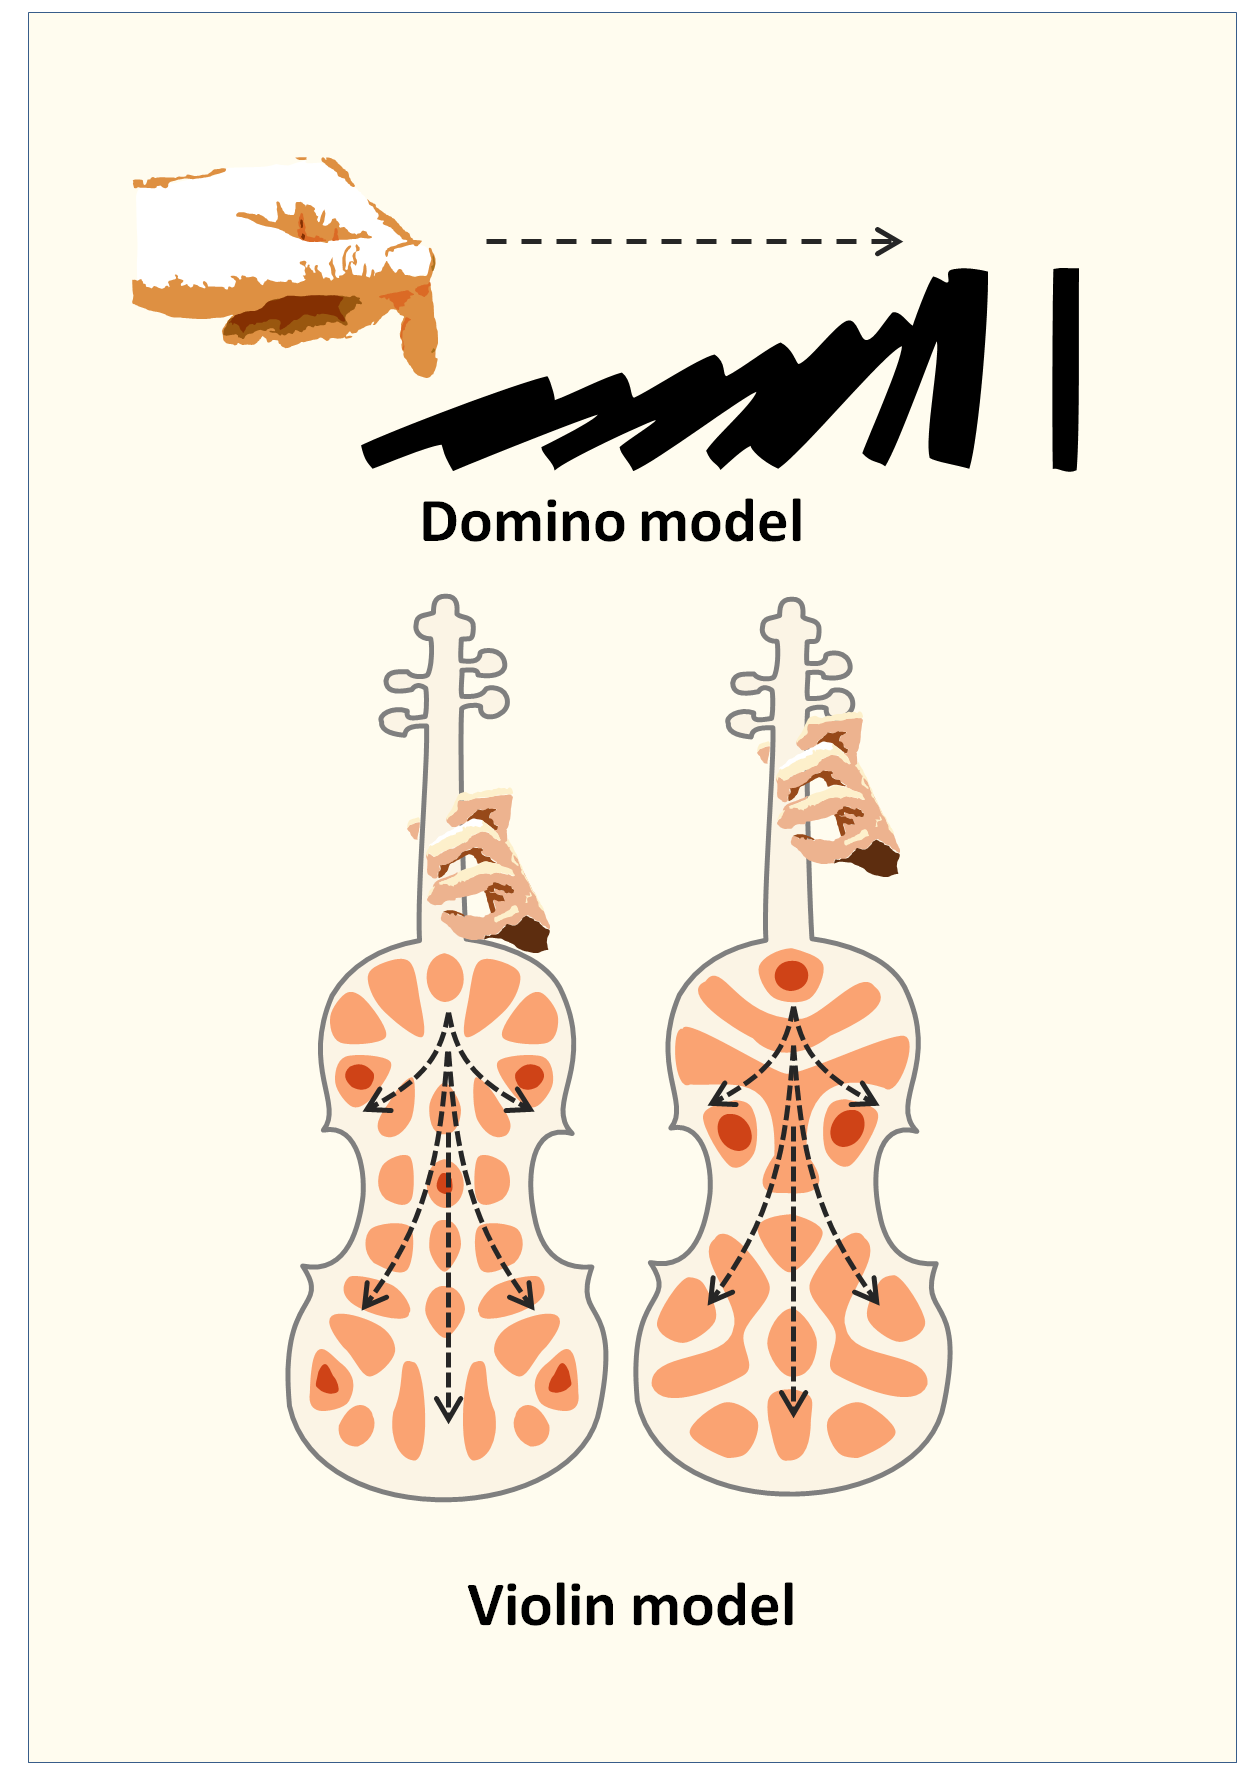
\includegraphics[width=0.5\textwidth]{./Figures/violin_metaphor.png}
\caption[``Domino" and ``Violin" Models of Signal Transduction]{When a small molecule binds to the allosteric site of a protein, information is transferred through the protein molecule to its active site. Two different methods of transmission can be defined. The first mechanism, here defined as the ``domino model", is a sequential set of events propagating linearly from the allosteric site to the active site. Binding of the effector triggers local structural changes that sequentially propagate via a single pathway to the active site. It was suggested that this mechanism is applicable for the PDZ domain family\cite{Lockless1999}, G protein-coupled receptors, the chymotrypsin class of serine proteases, and hemoglobin\cite{Suel2003a}. The second mechanism, defined here conceptually as a ``violin model", is based on vibration pattern changes inside the protein. In a violin its pitch can be changed by a slight movement of the violin player's finger on the fingerboard. Information about the finger movement is, thus, transferred throughout the whole body of the violin with no specific pathway for the signal transduction. By analogy, protein allosteric site is a fingerboard of the protein and a small signaling molecule is the player's finger. If a protein is in a particular vibration mode, it is possible to suggest that binding a small effector molecule to a specific site can change this mode. The signal, thus, will be spread throughout the whole protein including its active site. The ``domino model" is a reliable way to transfer information in a macro world, but on a molecular level, with significant thermal motions of the protein, this mechanism will be prone to random triggering of the domino chain reaction, creating noise in the signaling system. Thermal motions in case of the ``violin model" do not hinder the transduction. In fact, the permanent motion of the molecule is a prerequisite for this mechanism. Reproduced with permission from \citenum{Kornev2015a}. Copyright 2015 Cell Trends in Biological Sciences}
\end{figure}
\par Recent work has also revealed that protein allostery is not merely a transition between two discrete protein conformations, as initially thought, but rather a shift in the equilibrium populations of many conformations, induced by effector binding.\cite{Cooper1984a,Tsai2008a,Zhou2010b,Malmstrom2015,Pontiggia2015,Greives2014,Guo2015a} It is becoming increasingly clear that the kinetics of these transitions define the mechanisms of allostery.\cite{Zhou2010b,Malmstrom2015} Empowered with these new understandings and advances in molecular simulation (in terms of speed of calculation and improved methodologies), the era of allosteric drug discovery is now on the cusp of radical advancement.


\begin{figure}[htbp]
\centering
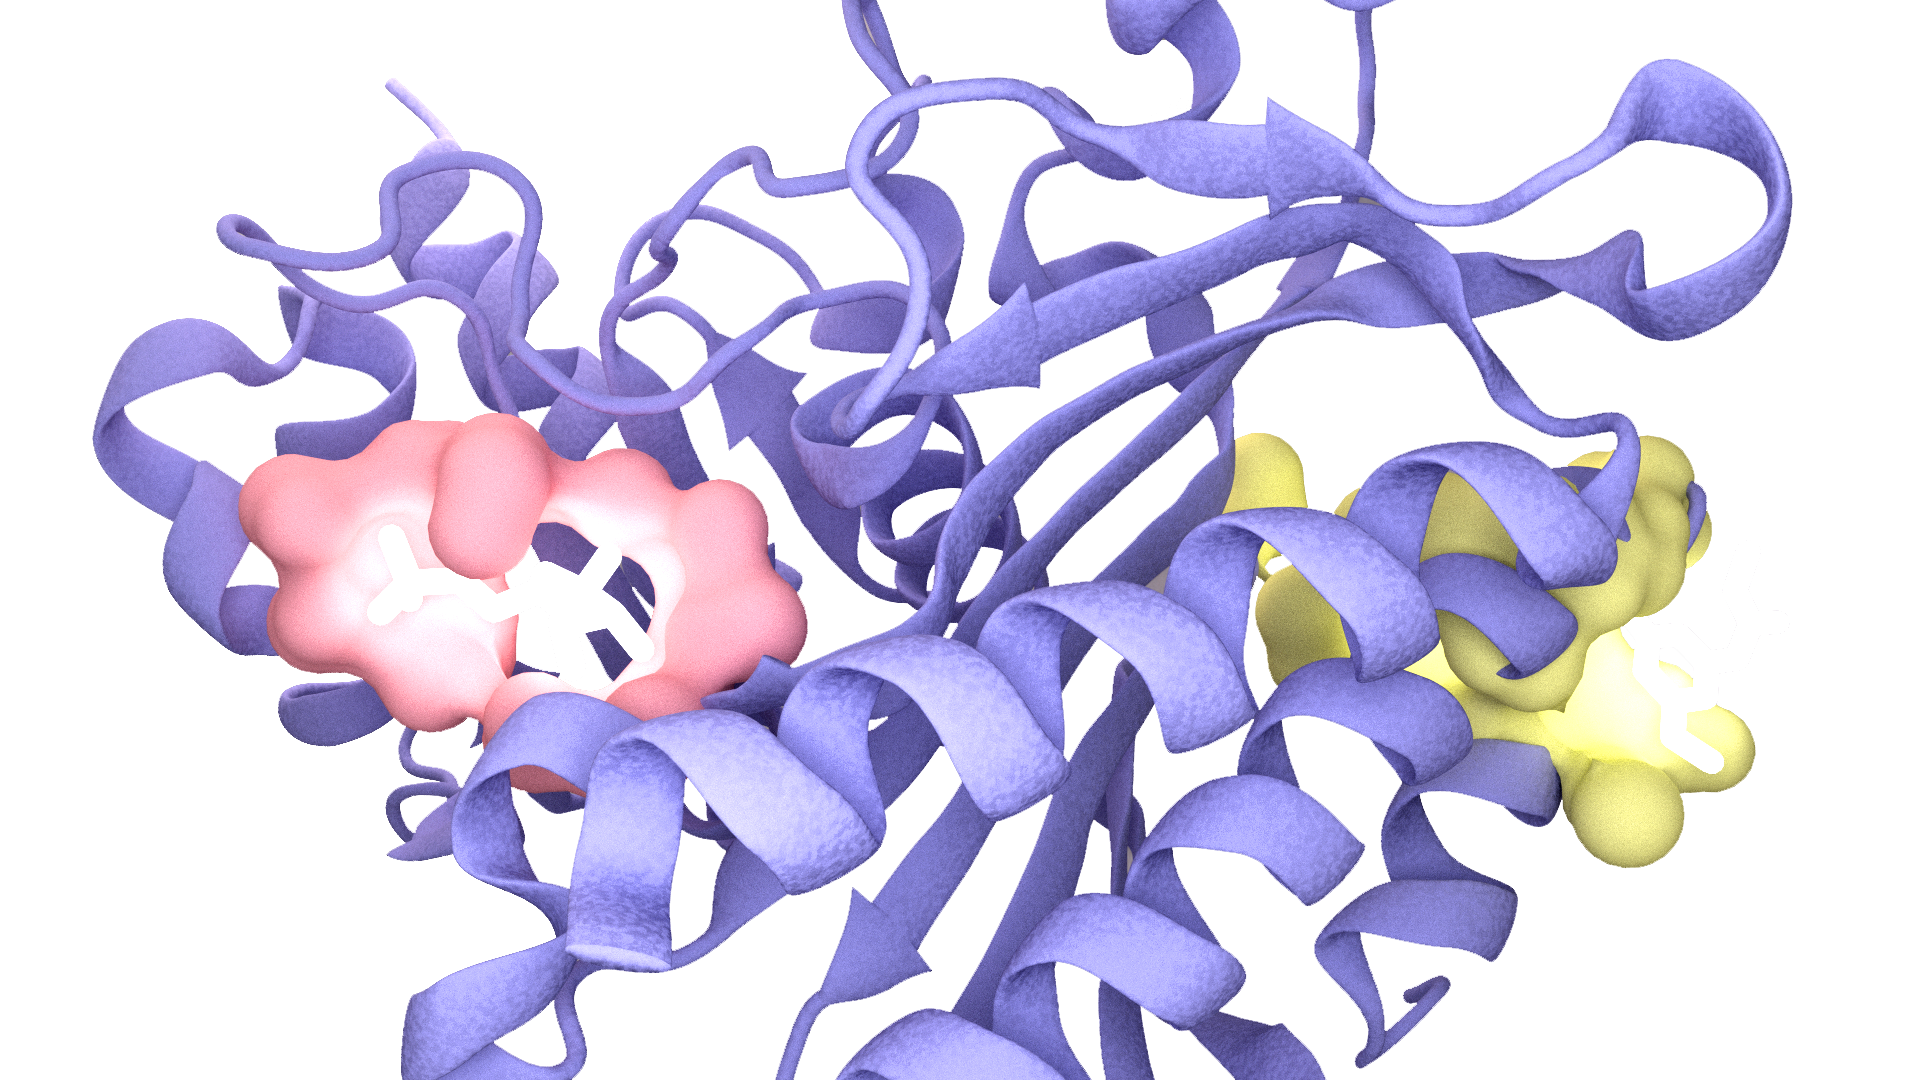
\includegraphics[width=\textwidth]{./Figures/allostery_example.png}
\caption[Orthosteric and Allosteric Sites]{The allosteric protein fructose 1,6-bisphosphatase, shown for illustration. Orthosteric and allosteric pockets (yellow and red, respectively) are bound to an endogenous ligand and an allosteric effector, respectively. Note that the allosteric site is distant from the orthosteric site such that there is no overlap between the bound poses of the allosteric and orthosteric ligands. Despite the distance between them, the allosteric effector measurably modifies the enzymatic activity at the orthosteric site. Illustration derived from PDB IDs 2Y5K\cite{Hebeisen2011a} and 3IFC.\cite{Zarzycki2011a}}
\end{figure}
\subsection{Emerging Rational Design Principles}
\par So-called tried-and-true ``design principles" are still being developed. However, a few general principles have begun to emerge. For example, many argue that it is insufficient to design a ligand that merely binds to an allosteric site; rather, the effector must make contact with certain key binding-pocket atoms to have the desired effect.\cite{Nussinov2012a,Wenthur2014} These key atoms can often be identified through mutagenesis experiments and crystallographic studies of other allosteric ligands.
\par A promising set of design principles is encapsulated in the ``allo-network" strategy, a rational approach that adopts two simultaneous but orthogonal approaches to ligand design.\cite{Szilagyi2013a} On the protein-structure level, the primary focus is to target a single protein function or an interaction with a single partner. On the signaling-pathway level, the ``allo-network" strategy suggests targeting less-connected upstream proteins instead of the more direct, though potentially highly connected, signaling proteins themselves. When applied to early-stage design, the allo-network method is predicted to increase the likelihood that a given allosteric effector will proceed through the drug-approval process.\cite{Nussinov2011,Szilagyi2013a,Csermelya2013}


\par Several published examples for recently approved allosteric drugs serve to illustrate the current state-of-the art for emerging allosteric drug design principles.  They also represent the significant advances that have been made to utilize structure-based methods for challenging druggable sites such as protein-protein interfaces and for membrane proteins such as ion channels. The available details of the discovery and optimization of these compounds do not include the methods discussed in this review, however they highlight where these predictive techniques could contribute to the allosteric design process.
\par In 2011, Gilmartin et al. of GlaxoSmithKline reported the discovery of a pharmacokinetically-optimized allosteric MEK inhibitor, GSK1120212.\cite{Gilmartin2011} The first generation inhibitor was discovered by high throughput screening \cite{Sebolt-Leopold1999} and the subsequent ternary crystal structure showed the allosteric pocket to be adjacent to the orthosteric ATP-bound site.\cite{Ohren2004} By 2012 there were fourteen allosteric MEK1/2 inhibitors in clinical trials,\cite{Zhao2014} because it was recognized that an inhibitor developed for this allosteric pocket afforded two very unique opportunities to avoid adverse clinical effects; the high doses required to compete against 1mM cellular ATP concentrations and inhibition of closely related ATP-binding sites in other kinases. The unique efficacy properties of GSK1120212 highlight both the opportunity and challenge of allosteric drug design.  Gilmartin et al. report that although some other MEK allosteric drugs demonstrate inhibition of the ERK1/2 pathway \textit{in vitro}, this has not translated into efficacy in patients.\cite{Gilmartin2011} GSK1120212  has since been approved in the U.S. under the name Trametinib for treatment of metastatic melanoma caused by the V600E mutation.
\par In 2012, Saalau-Bethell et al. of Astex reported the discovery of allosteric inhibitors for the HCV NS3 protein \cite{Saalau-bethell2012}. These inhibitors produce an allosteric effect by binding at an interdomain interface and stabilizing a pre-existing autoinhibited state of the protein. The original discovery of the allosteric site was accomplished using a fragment-based HTS technique, followed by optimization using X-ray crystallography and structure-based SAR. The authors discuss their experience with a few confounding factors in the allosteric design process, namely the need to use the full-length protein in their screening construct to observe the exerted allosteric effect, and the subsequent directed evolution study of resistance mutations that could occur at the allosteric site.
\par Hackos et al. of Genentech published on the discovery of positive allosteric modulators (PAMs) for GluN2A-containing NMDA receptors in 2016 \cite{Hackos2016}. PAMs are allosteric ligands which increase the effect of the endogenous signalling molecule and do not cause a change in its absence. The allosteric site in this case was at a protein-protein interface, and was discovered using HTS. Subsequent medicinal chemistry efforts then optimized the early hit molecule. The authors note that the validation of this allosteric site was reinforced by its similarity to an analogous allosteric site in AMPA receptors, but that the NMDA receptor site has elements of asymmetry that the AMPA receptor site did not. In comparing two similar compounds, GNE-6901 and GNE-8324, the authors make comments that indicate evidence of mode switching or a shallow SAR landscape, and they further characterize the details of the allosteric mechanism using mutagenesis experiments.
\par In summary these examples demonstrate allosteric drug discovery can be successful at protein sites often considered to be undruggable. It is apparent that these successes can be further built upon through computational methods that allow for rational rather than serendipitous HTS discovery of new allosteric binding sites and a deeper understanding of allosteric mechanisms that overcome design challenges such as mode switching.




\section{Computational Methods for Studying Allostery}
\subsection{Protein-Sequence Analysis Methods}
\subsubsection{Introduction}
\par Protein-sequence analysis is a useful tool to detect and characterize allosteric pathways and pockets. Here, we classify sequence-based methods into two groups: 1) \textbf{``single site"} methods, which produce a list of individual functional sequence positions; and 2) \textbf{``coupled site"} methods, which produce a list of groups comprised of two or more sequence positions that appear to be functionally linked based on their coevolution.
\par All sequence-based analysis methods share some challenges. These challenges include how to: select and aggregate clean, relevant sequences as input; interpret the output; and integrate sequence-analysis results with other forms of data. Determining the biological meaning of a strong signal is also problematic. While many analysis methods identify evolutionarily important residues, the specific biological role of these residues cannot be inferred without additional knowledge. For example, it is difficult to determine, based on sequence alone, whether an evolutionarily significant residue plays an allosteric role, or whether its role is related to another essential process (\eg substrate binding, maintaining protein structure, etc.).\cite{Talavera2015,Fodor2004c} Indeed, it is likely that a given residue serves multiple purposes simultaneously.
\par Input sequence selection and alignment also present challenges. Most techniques require many sequences to establish statistical significance. To obtain the required number of sequences, researchers often lower the stringency of their search parameters, resulting in alignments that contain sequences with lower similarity or incomplete coverage of the original query. While some analysis methods manage to detect meaningful coevolution over a wide range of multiple sequence alignment (MSA) conservation and noise levels, others are more susceptible to messy data.\cite{Fodor2004a,Johansson2010a} For a more complete discussion of these topics and how they affect coevolution analysis methods, readers are directed to an excellent recent review by Juan et al.\cite{Juan2013}
\subsubsection{Single-Site Evolutionary Analysis Methods}
\par By our definition, single-site evolutionary analysis methods return a list of predicted functional sequence positions but do not suggest specific linkages between sites. Once a researcher has constructed an MSA, the conservation or phylogenetic relevance of each column can be used to infer the evolutionary importance of each sequence position. This importance is sometimes a hallmark of thermodynamically critical residues that participate in allostery. Though single-site methods only return a list of single high-scoring sequence positions, the inner workings of some single-site methods are based on the aggregate or correlated behaviors of multiple sequence positions (\eg to determine baseline residue probabilities within a multiple-sequence alignment or construct a phylogenetic tree).
\par Single-site methods for detecting allostery are advantageous because they lack much of the noise often associated with correlation analysis. These analyses are also appealing because of their simplicity: There are usually fewer parameters to set, and the results can be visualized directly by highlighting key residues on a 3D protein structure.
\paragraph{Single-Position Entropy.} Shannon entropy, one of the simplest nontrivial sequence-analysis metrics,\cite{Shannon1948a} was used widely in early works to identify conserved sequence positions for drug-design or mutagenesis experiments.\cite{Shenkin1991a} Similar in form to thermodynamic entropy from statistical mechanics, Shannon entropy measures the population diversity of residues at a single MSA position. It is also central to mutual information (MI), a popular coupled-pair metric. The MI of two sequence positions is defined as the sum of the individual position entropies, minus the entropy of the positions considered jointly. While we not cover the mathematical details of these methods here, interested readers are directed to previous articles on these topics.\cite{Vinga2014a,Johansson2010a}
\par Shannon entropy does not consider amino acid similarity (\eg in the Shannon-entropy framework, a leucine-to-isoleucine mutation is considered mathematically equivalent to a leucine-to-arginine mutation). Other entropy measures, such as the relative Shannon entropy (also called the Kullback-Leibler Divergence (KLD)\cite{Kullback1951} and the von Neumann entropy,\cite{Zhang2008a,Peracchi2011} attempt to overcome this limitation and, as a result, may be more useful in the search for allosteric sites. Relative Shannon entropy/KLD accounts for some measure of the protein’s chemical environment by considering each mutation with respect to the background amino-acid frequencies calculated from the MSA. This analysis may be particularly useful when searching for allosteric sites in proteins that reside in membranes or other noncytosolic compartments, where background residue probabilities or mutational preferences may be biased due to different biochemical contexts. In contrast, von Neumann entropy, a concept borrowed from quantum statistical mechanics, is calculated using amino-acid similarity matrices. Identifying an optimal amino-acid similarity metric is nontrivial and may well depend on the nature of the system (\eg in a well-packed protein, residue size may be a sensitive metric, whereas surface-site comparison may require the user to prioritize charge). In a recent publication describing these types of entropy, Johansson and Toh explored how the two metrics can be mixed to detect enzyme active sites with maximum sensitivity.\cite{Johansson2010a}
\par Zhang et al. constructed a variety of new analysis methods in 2008 by combining Shannon or von Neumann entropy, phylogenetic tree structure, and a novel gap-treatment approach.\cite{Zhang2008a} In benchmarking their method, they compared their results to Evolutionary Trace and ConSurf (discussed in greater detail below). Two of their hybrid approaches outperformed all other techniques in detecting significant residues across a variety of proteins: the Improved Zoom method, which incorporates a tree breakdown of subalignments, and the Physiochemical Similarity Zoom method, which extends the Improved Zoom method with von Neumann entropy and tree-branch-size normalization.
\paragraph{Evolutionary Trace.} Lichtarge, Bourne, and Cohen pioneered the evolutionary trace (ET) method. The approach has become quite popular, largely because the algorithm is intuitive and its results are readily visualizable.\cite{Lichtarge1996} ET aligns a number of sequences and constructs a phylogenetic tree, then monitors the conservation of sequence positions at major tree branching points. By slicing the tree at different similarity cutoffs, the algorithm extracts the cluster-defining sequence positions. The evolutionary significance of these sequence positions is implied by their conservation in the sequences beyond the next branch. In their first paper,\cite{Lichtarge1996} the authors demonstrated that ET can detect functionally important sites in SH2, SH3, and DNA-binding domains. Work has since been published on ET validation, parameter optimization, and best-use practices.\cite{Madabushi2002a}
\par In a method often referred to as ``Difference-ET," the user runs ET on two related proteins and considers differences in the high-ranking residues and their scores. The sequence positions with strongly varying scores may suggest specificity determinants or differences in allosteric and/or orthosteric mechanisms. Notably, Difference-ET has been used in the study of GPCR specificity.\cite{Raviscioni2006a,Rodriguez2010a,Madabushi2004}
\par To better account for varying rates of evolution in different subtrees and correlated mutations, in 2004 Mihalek et al. developed real-valued ET.\cite{Mihalek2004a} This method incorporates entropy information into the standard ET framework. This work also introduces the zoom ET method (not related to Improved Zoom, above), which adds higher weight to sequences that are more similar to the protein of interest. In the introductory work, they used real-valued and zoom ET to detect the functional residues in a kinase domain, then compared the performance of both methods to regular (integer-valued) ET and entropy. Given unpruned sequence data sets, the real-valued ET and zoom ET methods outperformed the others by a significant margin. In contrast, integer-valued ET prevailed in most respects when pruned data was available. An automated web server is available to perform real-valued ET calculations, generate reports, and visualize results (\url{http://mammoth.bcm.tmc.edu/ETserver.html}).\cite{Mihalek2006a}
\paragraph{H2r(s).} In 2008, Merkl et al. introduced a method called H2r that serves as a segue between single-site and coupled-site approaches.\cite{Merkl2008a} H2r generates a mutual-information matrix for an MSA, then discards all but the strongest detected coupled pairs. For each sequence position $k$, the method returns $conn(k)$, the number of top-ranked pairs that include $k$. Initial work proved that H2r can successfully detect functionally significant residues across a range of proteins. More recently, H2rs, an improved version of H2r, has been released.\cite{Janda2014a} This method modifies the original by using von Neumann instead of Shannon entropy and performing more detailed checks for statistical significance. H2rs is available as a web server and a stand-alone application at \url{http://www-bioinf.uni-regensburg.de/}.
\subsubsection{Coupled-Site Evolutionary Analysis Methods}
\par Second-order sequence analysis detects residue pairs that mutate in concert more frequently than would be expected given random genetic events. Coevolving residue pairs are assumed to be functionally linked, often because they serve essential roles in allostery or structural integrity.
\par The immediate output of second-order allostery analysis is a list of residue pairs with associated correlation strengths. Combining these individual pairwise correlations into a single picture of the entire protein is a separate task. On the most basic level, the strongest correlations that include a residue or site of interest can suggest thermodynamic coupling to other sites, possibly related to allostery. More complex analyses use hierarchical clustering or principal component analysis to analyze these linkages and uncover strongly linked networks of coevolving residues.
\paragraph{Basic Coupled-Site Analyses.} Several simple yet reliable residue-coupling analyses have maintained a presence in the literature over the past decades. These basic approaches are advantageous because they are easier to understand and have been shown to score consistently well in a wide range of tests. However, they may fail to detect correlations in more complex cases.\cite{Pele2014a, Brown2010a} Though more complex methods exist, many of these basic methods still appear as analysis options in coevolution-detection software packages and web servers. In this review, we focus on a few that are still widely used.
\paragraph{Mutual Information.} Mutual Information (MI) is one of the most straightforward and long-lived coupling metrics. The MI between two sequence positions is defined as the sum of the Shannon entropies of both positions, minus their joint entropy. Due to its simplicity and favorable mathematical properties, MI analysis is the basis for a number of more complex coevolution methods. However, MI does present certain shortcomings. For example, uncorrelated pairs of high-entropy sequence positions are likely to have a higher MI than uncorrelated pairs of low-entropy positions.\cite{Simonetti2013a,Horner2007} To compensate for this and other shortcomings, various software packages have implemented a number of mathematical corrections to MI.\cite{Gao2011,Dunn2008,Wollenberg2000,Buslje2009a,Clark2014} Further, methods to estimate baseline values for correlation (e.g., resampling or sequence shuffling) can improve MI analysis.\cite{Martin2005,Crooks2004,Horner2007}
\par Another relatively direct coevolution metric, the McLachlan-Based Substitution Correlation (McBASC),\cite{Olmea1997} looks for similar patterns of variation in the columns of an MSA, weighting for residue similarity using the McLachlan scoring matrix.\cite{McLachlan1971} Analogous methods can be constructed using different substitution matrices, but McBASC continues to be a popular choice in the literature.\cite{Horner2007,Fodor2004a,Halperin2006}
\par In 2002, Kass and Horovitz\cite{Kass2002} analyzed the GroEL complex using a chi-squared test to detect significant residue coevolution in an MSA. The analysis suggested intra- and inter-chain contact pairs and has continued to appear in the literature under the name ``Observed Minus Expected Squared" (OMES).\cite{Horner2007,Ackerman2012,Pele2014a,Brown2010a,Fodor2004a}
\paragraph{Statistical Coupling Analysis.} The Statistical Coupling Analysis (SCA) method developed by Lockless and Ranganathan is perhaps the most widely used sequence-based method for allostery prediction.\cite{Lockless1999} SCA draws an analogy to statistical physics by calculating a ``coupling energy" between each sequence-position pair. The original SCA method computes a conservation value for each sequence position $i$ in an MSA, applies one of several types of perturbation to another position $j$ (depending on the SCA version,\cite{Ranganathan2012}) and finally recalculates the conservation at position $i$ for the sequences that satisfy the perturbation. By calculating the change in individual and joint conservation over a variety of perturbations, SCA establishes a ``coupling energy" that indicates the evolutionary coupling of positions $i$ and $j$.
\par The output of the SCA method is an $N\times N$ matrix of coupling energies, where $N$ is the number of sequence positions in the alignment. In early work, the researchers manually identified strongly coupled residue pairs that included one functional member (per experiment). More recent versions of SCA have grouped this matrix into meaningful clusters of coevolving residues using hierarchical or spectral clustering.\cite{Suel2003a}
\par Refinements of SCA have achieved improved statistical properties by resampling the original distribution.\cite{Halabi2009a} In a 2011 paper, SCA was effectively used to engineer a light-sensitive LOV2 domain onto the surface of DHFR at a location that SCA had identified as energetically linked to the enzyme active site. Some variants of the resulting protein chimera were found to have acquired light-dependent activity.\cite{Reynolds2011a}
\par Further work has used SCA to design artificial WW domains.\cite{Russ2005a,Socolich2005a} In 2011, an SCA analysis of antigen 85C from \textit{Mycobacterium tuberculosis} suggested new sites that potentially could be exploited in drug design.\cite{Baths2011a} A number of projects have also demonstrated how SCA can be used to target mutations that affect protein function.\cite{McLaughlin2012a,Peterson2004a,Hatley2003a,Shulman2004a,Smock2010a,Chi2008a,Fuentes2004}
\par Inspired by earlier work on the Sequence Correlation Entropy (SCE) method,\cite{Dima2004a} Dima and Thirumalai published an SCA variant in 2006.\cite{Dima2006a} This variant controls for specific protein composition by calculating the background probability that a given amino acid will be present at a random sequence position. This probability is determined by considering only the sequences being analyzed, as opposed to all sequences in the SWISS-PROT database.\cite{ODonovan2002a,Boeckmann2003a} Further, they borrowed a coupled two-way clustering procedure from gene-sequence analysis to define the sectors.\cite{Getz2000a} In validating this method, the authors analyzed the PDZ, GPCR, and lectin families of proteins and were able to quantitatively predict functional residues, which were in agreement with experimental findings.
\paragraph{Explicit Likelihood of Subset Co-variation.} As mentioned above, SCA is a ``perturbation-based" method in which correlation is established by excluding certain sequences from an MSA and monitoring how entropies change. Another popular perturbation-based method was published in 2003 by Dekker et al.\cite{Dekker2004} This method, Explicit Likelihood of Subset Co-variation (ELSC), relies on similar principles but returns correlation scores in the form of probabilities rather than statistical energies. ELSC was shown to be superior to SCA in contact prediction when tested on a range of protein families. It has since been implemented on web servers\cite{Yip2008,Kozma2012a} and has been a popular benchmark method in the literature.\cite{Halperin2006,Brown2010a,Ackerman2012,Pele2014a}
\paragraph{Direct Coupling Analysis.} In 2009, Weigt et al. proposed a mutual-information-based method called Direct Coupling Analysis (DCA) that disentangles directly interacting residues from large networks of indirectly coupled sequence positions.\cite{Weigt2008a} While this method is typically used in structure prediction to identify spatially adjacent sequence positions, it may find application in the study of short-range allosteric interactions. A more efficient implementation of the DCA method, known as ``mean field" (as opposed to the original ``message-passing" implementation) was published in 2011.\cite{Morcos2011a} Both introductory papers show that DCA is a robust predictor of both intra- and inter-protein contacts and that it can hint at the existence of unobserved protein conformations. Related work has shown that DCA can be used in conjunction with structural models to generate predictive models of protein complexes,\cite{Schug2009a,Sulkowska2012,Szurmant2013} determine the sequence positions that contribute to protein-interaction specificity,\cite{Procaccini2011a} and describe the conformational ensembles of proteins in crystallographic or near-crystallographic states.\cite{Morcos2013a} A web server and software package are available to perform DCA analysis at \url{http://dca.rice.edu/portal/dca/home}.
\paragraph{PSICOV.} PSICOV is another popular contact-detection method that may find productive use in the study of allostery.\cite{Jones2012a} Mathematically, PSICOV relies on an estimated inverse of the MSA covariance matrix, which acts as a matrix of correlations between all sequence-position pairs that inherently controls for the variations in all other positions. PSICOV was successful at predicting contacting protein residues based on MSA data. The code has been published online at \url{http://bioinfadmin.cs.ucl.ac.uk/downloads/PSICOV/}.
\paragraph{Recurrence Quantification Analysis.} Recurrence Quantification Analysis (RQA), another second-order sequence-analysis technique, is best used when much is already known about the mechanism under investigation (\eg physiochemical amino-acid properties such as charge or hydrophobicity are known to drive the allostery). RQA itself is a general method in nonlinear dynamics\cite{Eckmann1987a}: In the context of protein sequences, it considers a scalar-value vector that represents some property of a given sequence. In introductory work by Zbilut et al.,\cite{Zbilut1998a} the method was used to properly classify 56 TEM-1/\(\beta\)-lactamase mutants with impaired function based on their hydrophobicity profiles. Further RQA work used hydrophobicity scores to classify proteins as allosteric or nonallosteric,\cite{Namboodiri2010a} study p53 mutants,\cite{Porrello2004a} and reveal interaction partners in viral-envelope proteins.\cite{Giuliani2002a}
\par In 2005, Colafranceschi et al. investigated the effect of choosing different physicochemical amino-acid descriptors and changing the numerical parameters of the RQA algorithm.\cite{Colafranceschia} More recently, a comparison method based on RQA measurements, known as cross-RQA, effectively detected protein allostery.\cite{Namboodiri2012} Interested readers are directed to a review by Zbilut-Webber, which provides examples of RQA applied to a range of computational biology problems.\cite{Zbilut2002a}
\paragraph{Comparative Analyses.} Some work has been done to competitively benchmark the performance of these methods. In 2004, Fodor and Aldritch compared OMES, MI, SCA, and McBASC in a variety of tests. In short, the study found that performance is largely dependent on the way that different methods determine background residue probabilities and handle positional conservation.\cite{Fodor2004a} A follow-up study investigated how effectively coevolution analysis finds thermodynamically linked residue pairs.\cite{Fodor2004c} In general, spatially contiguous linked pairs were detected, but long-range couplings did not agree with experiments.
\par In 2010, Brown and Brown introduced a new pair-scoring method, called Z-scored-product Normalized Mutual Information (ZNMI), and compared it to the accuracy and reproducibility of MI, two versions of SCA, OMES, and ELSC.\cite{Brown2010a} The authors presented a thorough meta-analysis of method performance and the impact of input-parameter selection. Though none of the tools tested was particularly powerful, ZNMI was the most robust prediction tool. Brown and Brown also found that the use of multiple subalignments produced more accurate and reproducible results.
\par A comparative analysis of SCA and DCA revealed that the top 35 ``sectons" found via spectral clustering of the DCA matrix corresponded to pairs, triplets, and quadruplets of spatially contiguous residues.\cite{Rivoire2013a} In contrast, a similar analysis of the SCA matrix produced spatially adjacent clusters of many residues each. These different results validate the stated goals of each method: DCA aims to find contacting pairs, whereas SCA aims to find potentially distant groups that are thermodynamically linked in a certain function.
\par In 2014, Pel\'{e} et al. investigated seven coevolution analysis methods to find the hallmark covarying pairs in GPCR alignments.\cite{Pele2014a} They considered three variants of MI, McLachlan Based Substitution Correlation, SCA, ELSC, and OMES. OMES and ELSC were the most robust methods for finding the residues responsible for subfamily divergence. Their article also included an insightful discussion of the methods.
\par Mao et al. published a comparative analysis in 2015.\cite{Mao2015} Their study tests OMES, two variants of MI, SCA, PSICOV, and DI, and finds that PSICOV and DI are best at identifying contacting residues. OMES and MIp excel at removing false positives from the lists of predicted contacts. While the authors focused on detecting inter- and intramolecular contacts, their analysis also provided useful insights to guide the productive use of each method. For example, all methods benefit from repeatedly shuffling the MSA and rerunning the analyses in order to provide a baseline and remove false positives. Finally, the authors found that the consensus of DI and PSICOV provides a more robust prediction of contacting residues than any single prediction method alone. The software used to perform this analysis is available through the ProDy Evol program (\url{http://prody.csb.pitt.edu/evol/}).\cite{Bakan2011}
\par In the course of introducing new types of MI analysis (dbZPX2, dgbZPX2, and nbZPX2) and evaluating the effectiveness of MSA simulation (a topic beyond the scope of this paper), Ackerman et al. in 2012 compared many different coevolution analyses in their ability to predict contacting residue pairs.\cite{Ackerman2012} These comparisons found that the ``new" methods (the ZPX2 family, DCA, and log(R) (not discussed here)), were significantly superior to the ``old" methods (OMES, McBASC, ELSC, and SCA).
\paragraph{Web Servers.} Several web servers perform and visualize sequence analyses. Given a PDB code, Contact Map WebViewer (CMWeb)\cite{Kozma2012a} automatically constructs an MSA and visualizes a variety of coevolution analyses: mutual information, SCA, ELSC, OMES, and an early method presented by Gobel et al.\cite{Gobel1994a} The same server can also compare the results of these methods to user-uploaded data (\eg results the user obtained using some other type of analysis). The CMWeb server can be accessed at \url{http://cmweb.enzim.hu/}.
\par The Coevolution Analysis of Protein Residues server hosted by the Gerstein Lab\cite{Yip2008} (\url{http://coevolution.gersteinlab.org/coevolution/}) can perform a large number of the coupled-site analyses presented in this review, including SCA, ELSC, MI, and McBASC-type methods employing different scoring matrices. The server can also validate the results of these methods in predicting residue distances in a crystal structure.
\par MISTIC (Mutual Information Server to Infer Coevolution) is an automated web server that accepts user-submitted MSAs or collects them from PFAM.\cite{Simonetti2013a} MISTIC uses a corrected form of MI to infer coevolving pairs and offers several analysis methods that combine structure and coevolution.\cite{Buslje2009a} It can be accessed at \url{http://mistic.leloir.org.ar/}.
\par CAPS (Coevolution Analysis using Protein Sequences) is a unique algorithm that combines phylogenetic, 3D, and MSA data to predict coupled sequence positions.\cite{Fares2006a,Fares2006c} Versions 1 and 2 are hosted on web servers at \url{http://bioinf.gen.tcd.ie/caps/} and \url{http://caps.tcd.ie/}, respectively.
\par The Interprotein-COrrelated Mutations Server (I-COMS, \url{http://i-coms.leloir.org.ar/index.php}) focuses on detecting contacts at protein-protein interfaces, though it can also return intra-chain correlations.\cite{Iserte2015a} The server automatically builds alignments; performs MI, DCA, or PSICOV analysis; generates visualizations of the results; and allows users to download data taken from various points in the data-collection and analysis workflow.
\par In 2012, Jeong and Kim published a study describing a close MI variant.\cite{Jeong2012a} They employed an automated workflow to control for various types of noise in sequence alignments, using the MSA sequence profile to establish prior knowledge about the protein. While the authors only studied a few MI variants, they stressed that their profile-based method could be extended to more complex analysis techniques. Their approach, Correlated Mutation Analysis Tool (CMAT), is available on a web server at \url{http://binfolab12.kaist.ac.kr/cmat/}.
\par Access to ConSurf, a single-site detection method similar to ET, is available at \url{http://consurf.tau.ac.il/}.\cite{Berezin2004a,Glaser2003a,Landau2005,Armon2001,Ashkenazy2010a,Celniker2013a}
\paragraph{Software.} The ProDy Python package, referred to above, can compute a variety of coevolution metrics.\cite{Liu2010,Liu2012,Mao2015} In 2014, Skj\ae rven et al.\cite{Skjaerven2014} released the latest version of the powerful Bio3D R package for protein structure and sequence analysis.\cite{Grant2006a} While it focuses on structural analysis, the package can compute Shannon entropy and offers useful functions to create and manipulate sequence alignments. Also in 2014, Li et al.\cite{Li2014d} published the CorMut software package for R, which computes MI, a metric called the ``Jaccard index,"\cite{Rhee2007a} and the conditional selection pressure metric $K_a/K_s$.\cite{Hurst2002a}
\clearpage
\begin{sidewaystable}[htbp]
\footnotesize
\centering
\caption{A table of selected coevolution web servers/software packages and their capabilities}
\begin{tabular}{@{}p{2cm}|c|c|c|c|c|c|c|c|c|c|c|p{5cm}|p{5cm}@{}}
\hline
 &\turnme{Web server\,} & \turnme{Downloadable\,} & \turnme{Generates MSA\,} & \turnme{Shannon Entropy\,} & \turnme{Relative Shannon/KLD\,} & \turnme{MI\,} & \turnme{SCA\,} & \turnme{DCA\,} & \turnme{PSICOV\,} & \turnme{OMES\,} & \turnme{ELSC\,} & \turnme{Notes\,} & \turnme{URL\,}\\ \hline\hline
    CMWeb \cite{Gobel1994a} & X & X & X &  &  & X & X &  &  & X & X & Also computes an early method from Gobel et al. & \tiny{http://cmweb.enzim.hu/} \\ \hline
    MISTIC \cite{Simonetti2013a} & X &  &  &  & X & X &  &  &  &  &  & Calculates a corrected version of MI & \tiny{http://mistic.leloir.org.ar/} \\ \hline
    CMAT \cite{Jeong2012a} & X & X & X &  &  & X &  &  &  &  &  & Many noise-filtering parameters to customize; returns MI, MIp, and MIc & \tiny{http://binfolab12.kaist.ac.kr/cmat/} \\ \hline
    I-COMS \cite{Iserte2015a} & X &  & X &  &  & X &  & X & X &  &  & Offers two variants of DCA & \tiny{http://\mbox{i-coms}.leloir.org.ar/} \\ \hline
    ET \cite{Mihalek2006a} & X & X &  &  &  &  &  &  &  &  &  & Runs Evolutionary Trace & \tiny{http://mammoth.bcm.tmc.edu/ \mbox{ETserver.html}} \\ \hline
    Coevolution Analysis of Protein Residues \cite{Yip2008} & X & X &  &  &  & X & X &  &  & X & X & Also computes similarity matrix-based methods (including McBASC), Chi Square, and Quartets coevolution metrics & \tiny{http://coevolution.gersteinlab.org/} \\ \hline
    ConSurf \cite{Celniker2013a} & X &  & X &  &  &  &  &  &  &  &  & Performs a single-site type of analysis similar to ET & \tiny{http://consurf.tau.ac.il/} \\ \hline
    DCA \cite{Weigt2008a,Morcos2011a} & X & X &  &  &  &  &  &  &  &  &  & Returns pairwise DI & \tiny{http://dca.rice.edu/portal/dca/home} \\ \hline
    CAPS \cite{Fares2006a,Fares2006c} & X & X &  &  &  &  &  &  &  &  &  & Runs a nonstandard coevolution analysis technique & \tiny{http://caps.tcd.ie/} \\ \hline
    H2r \cite{Merkl2008a} & X &  &  &  &  &  &  &  &  &  &  & Runs a nonstandard single-site coevolution analysis technique & \tiny{http://\mbox{www-bioinf}.uni-regensburg.de/} \\ \hline
    H2rs \cite{Janda2014a} &  & X &  &  &  &  &  &  &  &  &  & Runs a nonstandard single-site coevolution analysis technique & \tiny{http://\mbox{www-bioinf}.uni-regensburg.de/} \\ \hline
    Bio3D \cite{Skjaerven2014} &  & X &  & X &  &  &  &  &  &  &  & R package; useful for creating and modifying sequence alignments & \tiny{http://thegrantlab.org/bio3d/} \\ \hline
    CorMut \cite{Li2014d} &  & X &  &  &  & X &  &  &  &  &  & R package. Also computes Ka/Ks and Jaccard index & \tiny{https://www.bioconductor.org/packages/ release/bioc/html/CorMut.html} \\ \hline
    ProDy \cite{Liu2010,Liu2012} &  & X &  & X &  & X & X &  &  & X &  & Python package; can compute DI and mutual information correction/normalization & \tiny{http://prody.csb.pitt.edu/evol/} \\ \hline
\end{tabular}
\end{sidewaystable}
\clearpage
\subsection{Simulation Methods / Correlated Motions}
\subsubsection{Molecular Dynamics and Monte Carlo Methods}
\par Protein allostery is intimately tied to protein dynamics. Allosteric effectors communicate with orthosteric pockets by altering protein dynamics, either through large-scale structural changes or more subtle changes in correlated residue motions. A proper understanding of the allosteric mechanism is impossible unless one fully appreciates the underlying dynamic conformational flexibility and energetic landscape.
\par Computational methods to characterize receptor flexibility include molecular dynamics (MD) and Monte Carlo simulations. Briefly, MD simulations represent molecular systems as beads (\eg atoms) connected by springs (\eg bonds). Newton’s equations of motion are numerically integrated to propagate the dynamics of this classically formulated system.\cite{Alder1959a,Rahman1964a,Karplus2002,Adcock2006} Simulation time is typically discretized into steps of one or two femtoseconds, as required to accurately simulate the fastest atomic motions (\ie hydrogen bond stretching). At each step, the potential energy of the system is calculated by considering the energies associated with bonded atoms (\eg due to bond stiffness, angle bending, torsion rotation, etc.) and nonbonded atom pairs (\eg due to electrostatic and van der Waals forces). The forces on each atom, calculated from the negative gradient of the potential energy, are then used to update the atomic positions at each step. In a related method, called ``accelerated MD" (aMD), \cite{Hamelberg2004,Wang2011,Miao2015a,Miao2015,Pierce2012a,Lindert2013a} the underlying potential energy landscape is modified by raising the energy wells. These modifications facilitate transitions between states that do not normally occur on the time scales of traditional MD simulations. Interested readers are directed to recent reviews that describe MD simulations in the context of drug discovery.\cite{Amaro2008,Amaro2010,Durrant2011b,Nichols2012a}
\par In contrast, Monte-Carlo-based methods take a stochastic approach to conformational sampling.\cite{Metropolis1953,HASTINGS1970} At each Monte Carlo step, a Markov-chain procedure is used to generate a slightly modified system conformation. This new conformation is then accepted or rejected at random, biased by the relative potential energy of the new conformation as compared to that of the previous step (the so-called ``Metropolis criterion."\cite{Metropolis1953}) As these simulations are stochastic, they do not typically explore conformational space via the same time-dependent path traced in an MD simulation. Indeed, a key limitation of the Monte Carlo method is that the time information connecting the states is lost. Nevertheless, Monte Carlo simulations are widely used because they tend to more efficiently sample system conformations that are statistically representative of the equilibrium state. A recently published book by Landau and Binder describes the technique in detail.\cite{Landau2009}
\subsubsection{Network Representations and Protein Allostery}
\par As mentioned above, allosteric signals can be transmitted through large-scale conformational changes or subtle shifts in the correlated motions/interactions of individual residues.\cite{Cooper1984a,Tsai2008a} Accessing the time scales required to observe many large-scale conformational changes is presently computationally intractable using unbiased simulation-based methods,\cite{Zwier2010,Noe2015} but these simulations are well suited to the study of allosteric signals that are transmitted via fast, local fluctuations (\ie nanosecond-scale changes in the coordinated motions of adjacent residues).
\par Distilling the dynamics sampled by these simulation-based methods into a simple  network representation of protein motions often facilitates allosteric analysis.\cite{Sethi2009,Gasper2012a,Freddolino2013,Yan2014,VanWart2012a,Ghosh2007,Collier2013} Rather than tracking the position of every atom, each protein constituent (\eg amino acid) is represented as a single node (located, for example, at the residue center-of-mass). Each pair of nodes is connected by an edge whose length is inversely proportional to the degree of interdependence between their motions, such that nodes connected by short edges are highly interdependent. Different metrics of ``interdependence" have been used, including metrics based on correlated motions (\eg mutual information,\cite{McClendon2009a,McClendon2012} fluctuations in atomic positions,\cite{Bradley2008c}, etc.) or the number of specific noncovalent interactions.\cite{Bradley2008c}
\par Once a network representation of protein dynamics has been constructed, various network-analysis techniques (described below) can identify important pathways of communication between distant residues that may contribute to allostery. Interested readers are directed to a recent review by Atilgan et al. for more detailed information.\cite{Atilgan2012}
\subsubsection{Dynamical Network Analysis}
\par A number of simulation-analysis techniques consider the interdependence of individual residues along an allosteric path or paths. In 2008, Bradley et al. analyzed molecular dynamics simulations of \textit{Escherichia coli} NikR, a transcriptional repressor of the NikABCDE nickel permease, using a novel network-space clustering approach.\cite{Bradley2008c} Two types of residue-residue interdependence were considered, based on fluctuations in residue motions and the number of polar contacts between residue-pair members. Bradley et al. first identified sets of residues whose motions and/or contact counts were correlated with residues in both allosteric and orthosteric pockets. These sets were then clustered using the ``unweighted pair group method with arithmetic mean" (UPGMA), a hierarchical agglomerative approach that groups residue sets according to the degree of similarity in their correlation patterns. The authors ultimately identified residue sets likely to mediate communication between the NikR allosteric \ce{Ni^{2+}}-binding pocket and the orthosteric DNA-binding pocket.
\par Others have pursued orthogonal methods to represent and analyze protein dynamics \textit{in silico}. In 2009, McClendon et al. introduced MutInf, a novel MD-analysis technique for identifying statistically significant correlated motions.\cite{McClendon2009a} Unlike other techniques, MutInf uses an internal coordinate scheme. Rather than considering the positional coordinates of residue atoms directly, it quantifies correlated motions using a mutual-information metric derived from residue torsion angles. This approach makes MutInf particularly well suited to study allosteric signals transmitted through the gear-like correlated motions of side-chain rotamers. Using multiple short simulations, the authors were able to identify statistically significant correlations. Applying the technique to interleukin-2 provided a viable theory of allosteric transmission involving a population-shift-mediated signal transmitted between the allosteric and orthosteric pockets via a hydrophobic core. More recent work has incorporated the Kullback-Leibler divergence metric to improve the sensitivity of MutInf analysis.\cite{McClendon2012}
\par A paper by Van Wart et al., published in 2012, studied imidazole glycerol phosphate synthase (IGPS), an important enzyme in the histidine biosynthetic pathway of plants, fungi, and microbes.\cite{VanWart2012a} Following a molecular dynamics simulation of the enzyme, they built a representative network of residue interactions as inferred by correlated motions. The edges connecting physically distant protein residues were ignored to emphasize correlations resulting from immediate physical interactions. The single shortest path (in network space) between the allosteric and orthosteric sites was then identified. Two of the residues along this path had been shown previously by experiment to be involved in allostery.
\par Van Wart et al. later expanded on their work by creating the freely available Weighted Implementation of Suboptimal Paths (WISP) program.\cite{VanWart2014a} WISP can identify not only the single optimal path connecting allosteric and orthosteric sites, but also multiple other near-optimal paths. While allosteric signaling may occur through a single optimal path in some cases, for many proteins it is likely the summed (or perhaps synergistic) effect of signaling through multiple near-optimal pathways.
\par While several efficient algorithms exist to calculate the single optimal path between two nodes in a network space (\eg the Floyd–Warshall algorithm, Dijkstra's algorithm, etc.), calculating near-optimal pathways is far more computation intensive. WISP uses several methods to first simplify the network representation of system dynamics. First, the edges between physically distant nodes are removed regardless of the interdependence of their motions, as in van Wart’s original paper. Second, all nodes that cannot possibly participate in optimal or near-optimal pathways of allosteric communication are deleted. For each node, Dijkstra's algorithm is used to calculate the shortest path connecting the source node, the node being considered ($n_i$), and the sink node. If this shortest path is still too long (in network space) to be an optimal or near-optimal pathway, no other path passing through $n_i$ can be optimal or near-optimal. Therefore, $n_i$ is deleted from the network. After thus greatly simplifying the network, it becomes computationally tractable to calculate notable pathways of allosteric communication between source and sink residues using a recursive, bidirectional approach.
\par In 2014, LeVine et al. introduced a novel analysis framework, called N-body Information Theory (NbIT), that uses multivariate mutual information to measure residue interdependence. This technique is unique in that it considers not only the interdependence (mutual information) between two residues, but also the mutual information between \textit{groups} of up to $N$ residues. Specifically, a metric called ``coordination information" is used to measure the degree to which the correlated motions of a set of residues are shared with another residue not in the set (\ie the ``contribution of a site to all possible \textit{n}-body correlations with another site"). The authors use this technique to analyze MD simulations of the bacterial transporter LeuT and identify many of the same residues previously found through experiment.\cite{LeVine2014a}
\subsubsection{Community Analysis}
\par A number of simulation-analysis techniques expand on calculations of residue-residue interdependence to consider how highly interconnected (and often rigid) \textit{communities} of residues interact with one another. In this view, allostery is achieved when largely isolated communities of highly interconnected residue nodes (``small-world networks") engage in long-range interactions. For example, in 2012, Rivalta et al. studied the allosteric mechanism of PRFAR binding to the IGPS heterodimer.\cite{Rivalta2012} After simulating the system in both the absence and presence of the allosteric modulator, they calculated the mutual information between the positional vectors of all residue-residue pairs. Ignoring the correlations between nodes that were not frequently physically adjacent ($\leq$ 5.0 \AA for at least 75\% of the simulation), the authors next used the Girvan-Newmann algorithm to identify communities of highly interconnected nodes. This analysis provides a powerful illustration of how an allosteric modulator might manipulate entire protein ``modules" to transmit a signal. Supported by NMR experiments, the authors ultimately concluded that PRFAR binding decreases the correlated motions at sideL of the heterodimer and induces conformational changes in sideR that ultimately impact the hydrogen-bond network near the active site.\cite{Rivalta2012} Sethi et al. used a similar technique in 2008 to study allostery in tRNA:protein complexes.\cite{Sethi2009}
\par The use of accelerated MD (aMD) simulations in this same mutual-information/community-analysis workflow has also proved fruitful. aMD simulations are particularly helpful when the allosteric mechanism being studied occurs on time scales that are longer than those accessible through traditional MD. For example, in 2012, Gasper et al. used a mutual-information/community-analysis technique to study $\alpha$-thrombin.\cite{Gasper2012a} Ultimately, their results suggested that $\alpha$-thrombin may have two allosteric pathways. One occurs on slower time scales that might not have been accessible were it not for the aMD. Others have used aMD to similarly study allosteric effects in the M2 muscarinic receptor.\cite{Miao2013a}
\par In 2014, Blacklock and Verkhivker used a similar technique to analyze MD trajectories of the Hsp90 chaperone in various functional states.\cite{Blacklock2014a} To verify the existence of communities in this system, they first calculated force constants for each residue, corresponding to the energy cost of residue displacement over the course of the equilibrium simulation. As residues with high force constants are typically rigid, community boundaries (\eg the boundary between a rigid module and a flexible inter-domain hinge site) often correspond to locations where these constants change abruptly. In fact, the ``hotspot" regions did correspond to residues known experimentally to be important hinge sites or sites of dimerization.
\par To further characterize this community-based organization, the authors next used protein-structure network analysis to build a network representation of Hsp90 dynamics. They calculated cross-correlation matrices from the MD simulations and identified residues with high degrees of ``centrality" (the number of interacting residues) and ``betweenness" (the frequency with which a given node lies along the shortest path in network space between two other nodes). Based on this analysis, the authors concluded that Hsp allosteric communication is mediated by highly stable central nodes, surrounded by residues with high degrees of betweenness that may ``shield" the more critical residues from the random Brownian/thermal motions common to all proteins.
\subsection{Pocket Detection}
\subsubsection{Introduction}
\par Simple pocket-finding techniques can be useful to identify potential allosteric sites. One straightforward approach is to consider any identified pocket other than the orthosteric to be allosteric. Pocket-detecting algorithms can be used to analyze static crystal structures. However, coupling these algorithms with techniques that account for pocket dynamics is often useful. Some allosteric pocket conformations are extremely rare in the absence of the allosteric effector itself. These ``cryptic pockets" are not readily evident in static apo- or ligand-bound crystal structures, but they may be predictively sampled with molecular dynamics simulations.\cite{Frembgen-Kesner2006,Bowman2012a,Wassman2013,Nair2014,Bowman2015b} Computational methods for pocket detection can be classified as geometry, knowledge, and energy based. We describe these three types of methods next.
\subsubsection{Geometry-Based Pocket Detection}
\par Geometry-based methods identify pockets by considering only the positions of the receptor atoms themselves. These methods are well suited to situations where speed of computation is critical (\eg when pocket detection is applied to conformations extracted from entire MD trajectories) or where pockets are particularly well defined. On the other hand, accuracy in pocket detection suffers when pockets are shallow, partially collapsed, or highly flexible. And pocket ranking by simple geometric metrics (\eg volume) does not always correlate strongly with ligand binding affinities or druggability because geometry-based methods do not consider the chemical properties of a given pocket.\cite{Durrant2011,Chovancova2012a,Eyrisch2007b,Brady2000a,LeGuilloux2009a,Schmidtke2011b,Halgren2007a,Halgren2009a,Brenke2009a,Votapka2013,Zheng2013a}
\par Many geometry-based algorithms have been described in the literature. They can be classified into three subcategories: sphere based, $\alpha$-shape based,\cite{Edelsbrunner1994a} and grid based. Sphere-based methods, such as PASS,\cite{Brady2000a} PHECOM,\cite{Kawabata2007a} POCASA,\cite{Yu2010a} and SURFNET,\cite{Laskowski1995a} first cover protein surfaces with spheres. Each sphere is evaluated and eliminated if judged unlikely to occupy a surface cavity. The locations of the remaining spheres identify likely binding pockets.
\par In contrast, methods such as  APROPOS,\cite{Peters1996a} CAST,\cite{Liang1998a} CASTp,\cite{Binkowski2003a} and Fpocket,\cite{LeGuilloux2009a} use $\alpha$-shape schemes to identify protein pockets. In brief, an $\alpha$-shape is like a convex hull, except that it potentially follows the surface of the source points more closely than a convex hull. The degree to which it deviates from the convex hull is controlled by the $\alpha$ value (for more details, see Edelsbrunner et al.\cite{Edelsbrunner1983a}). APROPOS compares multiple $\alpha$-shape representations of a protein at different values of $\alpha$.\cite{Peters1996a} Pockets are identified by subtracting ``higher-resolution" $\alpha$-shapes from ``lower-resolution" shapes. In contrast, CAST generates a Voronoi diagram based on protein-atom locations, removes any Voronoi edges and vertices that fall completely outside the receptor, and identifies pockets as collections of empty triangles (for details, see\cite{Liang1998a}). Fpocket uses a Voronoi tessellation to calculate receptor $\alpha$-spheres (\ie spheres that include four protein atoms on their surface but no protein atoms in their interior).\cite{LeGuilloux2009a} When clustered, these spheres tend to congregate at potential pocket sites.
\par Grid-based geometric methods for pocket detection include GHECOM,\cite{Kawabata2010a} LIGSITE,\cite{Hendlich1997a} LIGSITE$^{\textrm{CSC}}$,\cite{Huang2006a} POCKET,\cite{Levitt1992a} Pocket-Picker,\cite{Weisel2007a} PocketFinder,\cite{An2005a} Q-SiteFinder,\cite{Laurie2005a} and POVME/POVME Pocket ID.\cite{Durrant2014a,Durrant2011} These techniques consider points spaced along a grid that encompasses the protein receptor. Each point is evaluated for the likelihood of pocket occupancy, and high-scoring points are clustered to identify binding pockets, whether orthosteric or allosteric. Various metrics are used to evaluate the points, depending on the algorithm. They include the presence of steric clashes with the protein, detected protein-solvent-protein events,\cite{Levitt1992a,Hendlich1997a} buriedness indices,\cite{Weisel2007a} predicted methyl-probe interaction energies,\cite{Laurie2005a,An2005a} etc.
\par As a representative example of the geometry-based class, consider POVME/POVME Pocket ID, a grid-based pocket-finding algorithm.\cite{Durrant2014a,Durrant2011} POVME Pocket ID identifies surface and internal cavities by first creating a low-resolution 3D grid of equidistant points that encompasses the entire protein. Points are removed if they are physically near any protein heavy atom or fall outside the convex hull defined by the protein $\alpha$-carbons. The volumes corresponding to the remaining low-resolution points, which tend to encompass protein pockets, are then replaced with smaller, higher-resolution 3D grids, and the same point-eliminating process is repeated. Finally, any remaining high-resolution points that have fewer than a user-defined number of neighbors are eliminated iteratively until no such points remain, and stretches of contiguous points are grouped together into distinct pockets.
\par The locations of these identified pockets can be fed into the POVME program, which calculates pocket metrics such as volume and shape. The latest version of POVME can efficiently analyze entire MD trajectories, allowing the user to monitor pocket changes over time and identify sampled conformations that are geometrically distinct. This approach is useful for identifying cryptic pockets that only occasionally manifest themselves over the course of an MD simulation.
\subsubsection{Knowledge-Based Pocket Detection}
\par Knowledge-based algorithms draw on large structural and genomic databases to determine binding-pocket locations based on sequence and overall structure rather than pocket shape. Algorithms such as 3DLigandSite,\cite{Wass2010a} FINDSITE,\cite{Brylinski2008a} and Pocketome\cite{Kufareva2012} infer these locations by querying existing databases for ligand-bound proteins that are structurally similar to the target protein. These algorithms work particularly well when the target protein has a highly conserved binding site. Other methods, such as FRpred, use sequence conservation, in conjunction with supporting methods like surface-residue-prediction algorithms, to identify surface residues that are likely biologically important.\cite{Fischer2008a} Finally, some hybrid methods, such as the evolutionary-trace method,\cite{Lichtarge2002a} ConSeq,\cite{Berezin2004a} and ConCavity,\cite{Capra2009a} combine sequence and structural homology to identify likely binding pockets. The ``Single-Site Evolutionary Analysis Methods" section above describes methods like these in further detail.
\subsubsection{Energy-Based Pocket Detection}
\par Energy-based methods identify binding sites by evaluating whether or not a given protein region interacts favorably with docked small organic probes. These methods are particularly useful to detect a given pocket \textit{and} assess its druggability. This additional information does come at a cost; energy-based methods are more computationally demanding and so do not scale well, limiting their applicability when analyzing large-scale structural datasets or MD trajectories.
\par Methods such as SiteMap\cite{Halgren2009a} and SITEHOUND\cite{Hernandez2009a} use single probes (typically methane or water molecules) to assess the likelihood of small-molecule/protein binding. In contrast, methods such as FTMap,\cite{Kozakov2011a,Kozakov2015a,Brenke2009a} GRID,\cite{Goodford1985a} and MCSS\cite{Miranker1991a} consider multiple chemically diverse probes and so identify not only pockets, but druggable hot spots that are more likely to function as orthosteric or allosteric binding sites.
\par FTMap\cite{Kozakov2011a,Kozakov2015a,Brenke2009a} in particular warrants further discussion. FTMap is the computational equivalent of the Multiple Solvent Crystal Structures (MSCS) technique.\cite{Allen1996,Mattos1996a} Rather than superimposing multiple crystal structures obtained by soaking a protein in 6-8 different organic solvents, FTMap computationally docks 16 distinct organic probes into a user-provided protein model. The docked positions of these probes are then clustered, and the clusters are ranked by their Boltzmann-averaged energies. In an alternate implementation called FTSite,\cite{Ngan2012a} adjacent, mutually accessible clusters are combined into ``sites" that are then ranked by the number of nonbonded contacts between the protein and the corresponding probes. Both these techniques can be applied to multiple structures, whether derived from X-ray crystallography or simulation, to potentially identify cryptic sites that are not always evident when single structures are considered. FTMap can be used to identify possible allosteric sites. For example, Ivetac et al. used it to detect five potentially druggable sites on \(\beta_1\)AR and \(\beta_2\)AR.\cite{Ivetac2010a,Ivetac2012} It has also been used to evaluate the druggability of p53 cryptic pockets, which were subsequently used to prospectively discover novel reactivation compounds.\cite{Wassman2013}
\subsection{Markov State Models}
\subsubsection{Introduction}
\par Over the past 10 years, Markov state models (MSMs) have been used increasingly to analyze molecular dynamics simulations, suggesting that they are already promising tools to study allostery in a drug-discovery context.\cite{Pande2010a,Schwantes2014a,Chodera2014a,Malmstrom2014,Shukla2015,Bowman2015b} In brief, a Markov state model is a stochastic kinetic model that describes the probability of transitioning between discrete states at a fixed time interval.\cite{Beauchamp2011a,Pande2010a,Prinz2011c} These models are required to have the Markovian property (\ie thatvthe probability of transitioning between discrete states is independent of previous transitions).


\par By clustering protein structures extracted from an MD trajectory, it is possible to identify discrete conformational states for use in MSMs.\cite{Beauchamp2011a,Pande2010a,Prinz2011c} Transitions between conformational clusters observed over the course of an MD trajectory are tallied, and the MSM is then built from the transition probabilities between these distinct clusters. As they are built solely on these transition probabilities, MSMs can draw upon multiple trajectories, enabling efficient sampling of the entire conformational space through many independent simulations carried out in parallel. MSMs can be built with the software package MSMBuilder, available at \url{http://msmbuilder.org/latest/}.\cite{Beauchamp2011a} EMMA\cite{Senne2012}, available at \url{http://www.emma-project.org/latest/}, is another useful building tool. Because independent trajectories are aggregated as a post-processing step, the simulations can be carried out on a variety of computational resources, including independent desktop machines, local clusters, or high-performance computing resources. A recent example carried out by Kohlhoff et al. used tens of thousands of trajectories carried out on Google’s exascale cloud computing resources. By subsequently ``knitting together" the simulation data within a MSM framework, the researchers elucidated the activation pathway of GPCR $\beta_2AR$.\cite{Kohlhoff2014}


\par MSM/MD analysis provides access to the thermodynamic, kinetic, and structural characteristics of the protein conformational ensemble (\ie a robust description of the free-energy landscape of the protein).\cite{Beauchamp2011a,Prinz2011c,Prinz2011d,Senne2012,Cronkite-Ratcliff2013a,Pande2010a} The thermodynamics of the various conformational states can be calculated from the equilibrium distribution. It is also possible to resolve the transition kinetics between individual states, the concerted or principal protein motions, metastable states, and the transition pathways between discrete states.\cite{Prinz2011d,Senne2012,Beauchamp2011a} Lastly, the MD trajectories also provide representative receptor snapshots for use in structure-based drug design.\cite{Cronkite-Ratcliff2013a}
\subsubsection{MSMs and Drug Discovery}
\par MD-based MSMs were originally developed to study protein folding,\cite{Lane2011a,Bowman2010a,Lapidus2014a,Schwantes2014a,Li2014f,Schor2015a,Voelz2010c} but they can also be used to study molecular phenomena that are directly applicable to allostery and drug discovery, including cryptic site identification,\cite{Bowman2012a,Bowman2015b,Kohlhoff2014} protein-ligand interactions,\cite{Buch2011,Tiwary2015} and  protein function.\cite{Lane2011a,Kohlhoff2014,Vanatta2015,Malmstrom2015}
\par MSMs have been used to study binding-site conformational heterogeneity, revealing conformations that are not readily evident in any crystal structure. In 2012, Bowman and co-workers used MSMs to identify and validate cryptic allosteric sites in TEM-1 $\beta$-lactamase, interleukin-2, and RNase H.\cite{Bowman2012a,Bowman2015b} Similarly, in a recent study of GPCR conformational transitions, Kohlhoff et al. identified intermediate conformations that they used successfully in a subsequent virtual-screening campaign.\cite{Kohlhoff2014} Shukla and co-workers also identified a key conformational intermediate in the Src kinase activation pathway that could be used as a target for drug discovery.\cite{Shukla2014b} While traditional molecular dynamics simulations have been used to identify cryptic allosteric sites and elucidate binding-site conformational diversity, Markov state models can characterize the probability and dynamics of these conformations, permitting rational design against dynamic pockets.
\par Researchers have also employed MSMs to gain insights into ligand-protein binding that are critical to both allosteric and orthosteric structure-based drug discovery. Buch et al. used MSMs derived from multiple independent MD simulations to accurately determine the $k_{on}$ and binding free energy of benzamidine to trypsin.\cite{Buch2011} Building on that work, Tiwary et al. used MSMs in conjunction with metadynamics, a variant of molecular dynamics, to determine the $k_{off}$ for the same system.\cite{Tiwary2015} While this approach is currently too computationally demanding for virtual screening, it has identified transitory sites important for binding and shed new light on the interactions that govern ligand-binding kinetics.


\par MSMs also provide useful insights into how a protein conformational ensemble begets function and transmits allosteric signals. Most studies have focused on the transition between two functional states. In this context, MSMs have been used to study Src kinase,\cite{Shukla2014b} the \(\beta_2\) adrenergic receptor (\(\beta_2\)AR),\cite{Kohlhoff2014} and bacterial response regulator NtrC.\cite{Pontiggia2015,Vanatta2015} Malmstrom et al. recently used this same technique to study allostery in the cyclic-nucleotide binding domain (CBD) of protein kinase A.\cite{Malmstrom2015} By building and simulating models of the CBD, with and without bound cAMP, the study provided insight into how ligand binding modulates the protein conformational ensemble.


\par As it is challenging to determine the impact of an effector molecule on the conformational ensemble, most MSM studies to date have not examined allostery directly. Nevertheless, two relevant themes emerge from existing studies. First, kinetics play an important role in the transition between functional states.\cite{Malmstrom2015,Pontiggia2015,Vanatta2015} This is best shown in our study of the PKA CBD, where the effector molecule cAMP significantly modulates the kinetics of the transition from the active to the inactive states of the protein, while simultaneously leaving the reverse transition between the inactive and active states unmodified.\cite{Malmstrom2015} This modulation seems to be regulated by transient interactions between the effector molecule and the protein. Second, recent MSM studies suggest that there is not one but many pathways between functional states. Studies of \(\beta_2\)AR,\cite{Kohlhoff2014} NtrC,\cite{Vanatta2015,Pontiggia2015} and the PKA CBD\cite{Malmstrom2015} each revealed multiple transition pathways that arose from transient interactions within the system, suggesting a probabilistic model of allostery in addition to one that describes allostery in terms of concerted pathways.\cite{Vanatta2015} Studies like these can provide useful insights applicable to structure-based drug discovery targeting transitional conformational states.


\par MSMs can provide significant insights into protein-ligand interactions and allostery, but building these models is computationally demanding, limiting their use as screening tools. This weakness aside, MSMs do provide a strong foundation for rational drug discovery and enhanced understanding of allosteric mechanisms.


\section{Energy Landscape and Topological Analyses}
\subsection{Introduction}
\par Like MSMs, energy-landscape theories were originally developed to study protein folding. But they too can be applied to the study of allosteric mechanisms and protein dynamical modes. Per statistical mechanics, the underlying free-energy landscape of a system determines the probability of observing a particular configuration. Any topological analysis aimed at understanding allostery must be based on a thermodynamic understanding of the impact that effector binding has on this energy landscape.
\subsection{Protein Frustration}
\par It is helpful to view allosteric binding as an event that perturbs the conformational exchange, or folding pathways, of a protein. The principles of statistical mechanics applied to polymers in solution have provided much insight into the protein-folding process. As proteins fold, the number of native contacts increases, and the entropy of the polymer decreases. Folding is impossible when the required conformational transitions are occluded by large free-energy barriers or wells. For example, a large local minima along the folding pathway could force a protein to undergo a glass transition, leading to a kinetically trapped state. Typical folding must be governed by the ``principle of minimum frustration" (\ie the folding pathway must be funnel shaped and relatively smooth). \cite{Bryngelson1987,Wolynes1995,Onuchic1996,Onuchic1997b,Wolynes2005,Karplus2011}
\par In terms of allostery and energy-landscape theory, a positive allosteric modulator can be seen as a compound that increases the likelihood of the binding state by deepening the binding-state well or decreasing the depth of competing wells. On the other hand, a negative allosteric modulator may shift the location of the binding-site well, shallow out the well, or increase the depth of competing wells. Using these guiding principles, heuristics can be designed to identify each of the above scenarios.
\par Ferreiro et al. have developed a heuristic to pick out locally frustrated residues.\cite{Ferreiro2007a,Ferreiro2011a} While the overall folding process obeys the principle of minimum frustration, this does not preclude the possibility of having small local barriers that must be overcome to fold. To detect these local frustrations, the authors systematically perturbed the amino-acid sequence and compared the perturbed total energy with that of the native state. This comparison provided the effective stabilization energy associated with each amino-acid pair. If a given native-state interaction is highly stabilizing (\ie the interaction energy is favorable compared to mutants), it is said to be ``minimally frustrated." On the other hand, if a pair of residues is sufficiently destabilizing (\ie the interaction energy is weak compared with that of the mutants), it is ``frustrated." Frustrated residues can be thought of as weak points in the global structure, contributing to barriers that may introduce slow degrees of freedom. As such, they may be involved in ligand binding or allostery. Jenik et al. have implemented this heuristic as a web server \url{http://www.frustratometer.tk/}.\cite{Jenik2012}
\par Weinkam et al. used a dual-topology G\~{o} model\cite{Go1984a} to survey the free-energy landscape of the calmodulin-GFP \ce{Ca^{2+}} sensor protein, the maltose binding protein, and the CSL transcription factor. They introduced a truncated Gaussian distance term to the soft-sphere atom overlap term implemented in MODELLER,\cite{Sali1993a,Marti-Renom2000a,Fiser2000a,Eswar2007a} resulting in either one basin corresponding to the bound/unbound distances or two corresponding to both, depending on the pairwise distance and cutoff. Subsequent MD simulations of the resulting model were analyzed using their pseudocorrelation map algorithm.\cite{Weinkam2012a} They found that their model reproduces allosteric motions and sheds insight into the macroscopic mechanism.
\subsection{Normal Mode Analysis}
\par Protein dynamics and subsequent perturbations from binding events can also be studied using normal mode analysis (NMA).\cite{Bahar2005a,Zheng2006a,Zheng2009c} NMA assumes that the potential energy landscape in the vicinity of a minimized atomic structure is approximately harmonic. This simplifying assumption allows for diagonalization of the Hessian matrix. Solving the eigenvalue problem produces the eigenvectors (movement direction) and eigenvalues (vibrational frequencies). NMA is known to reproduce the slow degrees of freedom of protein motion well.\cite{Ma2005a,Bahar2005a} Applying additional constraints to simulate the impact of an effector on binding-site residues can yield new fundamental modes that may provide insight into the allosteric mechanism.
\par Ming and Wall applied normal mode analysis to investigate the effect of tri-\textit{N}-acetyl-\textsc{D}-glucosamine upon lysozyme.\cite{Ming2005c} They assumed that greater perturbation to the conformational distribution corresponds to increased likelihood that a binding event will occur at a regulatory or active site. The degree of perturbation is monitored by comparing the distributions predicted by NMA of the protein with and without the ligand bound, via the Kullback-Leibler Divergence. In this work, Ming and Wall generated many arbitrary poses and investigated the allosteric potential, defined by the KLD. They showed that sites with large KLD correspond with identified functional lysozyme residues.
\par The use of normal mode analysis removes the need to integrate the equations of motion. However, for the harmonic approximations to be accurate, the starting structure needs to be in a local minima. An initial molecular mechanics minimization can ensure that proteins of interest are near what might be seen in their native environments (\eg a GPCR embedded in a lipid bilayer with heterogeneous composition). However, alternate options include simplified interaction hamiltonians such as those offered by elastic network models (ENMs).
\paragraph{Elastic Network Models.} The complexity and computational cost of simulating detailed atomic potentials inspired development of simpler ENMs in which uniform harmonic potentials are used to model all interactions.\cite{Tirion1996a,Bahar1997a,Haliloglu1997a} A popular ENM is the Gaussian Network Model (GNM), wherein neighboring residues are connected by virtual springs to create a network/graph of interactions. Here the interatomic potential energy, $U$, of the system can be expressed as,
\begin{equation}
    U = \frac{\gamma}{2}\left[\sum_{i,j}^{N}\delta R_i\Gamma\delta R_j\right],
\end{equation}
where $\gamma$ is the uniform force constant of the harmonic springs, ${\delta R}$ is the $N$-dimensional column vector of the instantaneous fluctuations of specific atoms, and $\Gamma$ is the $N\times N$ Kirchoff (connectivity) matrix of residue interactions given by,
\begin{equation}
    \Gamma_{ij} = \begin{cases}
        -1, & \text{if } i \neq j \text{and } R_{ij} \leq R_c\\
        0, & \text{if } i \neq j \text{and } R_{ij} > R_c\\
        -\sum_{i,i\neq j}^N \Gamma_{ij}, & \text{if } i = j
    \end{cases}
\end{equation}
where $R_c$ is a residue cutoff distance.
\par Ming and Wall have developed a backbone-enhanced elastic network model (BENM) in which the interactions between connected residues are scaled by an additional factor. Using an objective function defined by the KLD of the marginal distribution of all-atom and $C_{\alpha}$ atomic coordinates, the authors showed that BENM can reproduce the atomistic mean-squared displacement for bovine pancreatic trypsin inhibitor (BPTI).\cite{Ming2005a} To consider the effects of allostery, the authors again used the KLD of local conformational distributions before and after ligand binding.\cite{Ming2005a}
\par To locate allosteric binding sites, Su et al. recently identified allosterically coupled regions in a GNM using a thermodynamic method.\cite{Su2014c} All neighboring residues (represented by their corresponding $C_{\alpha}$ atoms) were connected by virtual harmonic springs of equivalent strength. A spherical probe then sampled the protein surface to locate the potential effector interaction points. Additional springs were attached between the effector point and the local residues in the protein-effector model. The free-energy difference ($\Delta\Delta G$) between the protein-ligand and protein-effector-ligand systems was calculated. Regions with large $\Delta\Delta G$ values were assumed to be important for the allosteric mechanism. Using this method, Su et al. studied the Hsp70 and the GluA2 AMPA receptors. These allosteric predictions corresponded to experimental results.\cite{Su2014c}
\par Berezhovsky et al. used a similar coarse-grained network-interaction model to predict the location of allosteric sites.\cite{Berezovsky2013a} To identify potential pockets for effector/substrate binding, the authors generated a ``residue interaction graph" (RIG), with residues as nodes and interatomic contacts as edges. They then evaluated the ``local closeness," defined as the number of total neighboring residues weighted by $1/r$, where $r$ is the inter-residue distance.\cite{Mitternacht2011b} Regions with high local closeness were likely to be in pockets and, thus, were putative binding sites. The extent to which each binding site was coupled to the intrinsic protein motions was then explored by estimating the strain (so-called ``binding leverage") on ligand-protein contacts under deformations described by NMA. A ligand that bound to a site with high binding leverage could restrict protein dynamics.\cite{Mitternacht2011a}
\par The binding leverage describes the extent to which changes in binding sites and protein conformational degrees of freedom are coupled; it does not specifically predict allosterically linked sites. To predict allostery, Mitternacht and Berezovsky introduced ``leverage coupling," which selects for sites that are strongly coupled to the same degree of freedom.\cite{Mitternacht2011a} The mode associated with the most binding leverage is considered most relevant, based on the assumption that there is one dominant motion promoting allostery. These methods have been implemented in the online SPACER server \url{http://allostery.bii.a-star.edu.sg/}.\cite{Goncearenco2013a}
\section{Conclusions}
\par Over the past decade, advances in computing power and predictive algorithms coupled with the increased availability of structural and biochemical data have revealed new opportunities for rational design of allosteric drugs. The emergence of novel computational approaches to describe and predict allosteric phenomena across a range of scales, from the coordinated atomic movements in a single receptor molecule to complex allosteric signaling networks, is ushering in a new era wherein computational methods can be used to prospectively predict, discover, and characterize allosteric sites and effector molecules. Within the context of a drug-discovery program, such approaches hold the potential for developing drugs with increased specificity and selectivity, as well as the ability to gain new and more comprehensive understanding of old targets. For example, the convergence of advances in (i) theoretical MSM-based frameworks and MSM building software, (ii) community MD codes that can achieve $>100$ ns/day sampling for realistic sized systems on single gaming/commodity GPU processors, and (iii) pocket and druggable site-detection algorithms now make it possible for researchers even in industrial settings, with fast-paced timelines and stringent quality standards, to apply these approaches to drug targets already in their arsenals. The application of these methods to kinases and GPCRs seems particularly worthwhile, given the existence of assays and structural data, and the challenges faced by existing drug candidates in the clinic.
\section{Acknowledgements}
\par \cref{chap:allostery}, in full, is a modified reprint of the material as it appears in ``Wagner, J. R.$^{\dagger}$; Lee, C. T.$^{\dagger}$; Durrant, J. D.; Malmstrom, R. D.; Feher, V. A.; Amaro, R. E. \emph{Emerging Computational Methods for the Rational Discovery of Allosteric Drugs.} Chem. Rev. 2016, 116 (11), 6370–6390.''.
The dissertation author was a primary coinvestigator and author of this work.

\par This work was funded in part by the Director's New Innovator Award Program (NIH DP2 OD007237 to REA) and the National Science Foundation through XSEDE supercomputer resources provided via TG-CHE060073N to REA. Funding and support from the National Biomedical Computation Resource was provided through NIH P41 GM103426. JRW and CTL are supported by a NIH Molecular Biophysics Training Grant T32 GM008326. Additional resources from the UC San Diego Center for Drug Discovery Innovation and the Keck II Computing and Visualization facility are gratefully acknowledged.
